\documentclass{beamer}
\usepackage{beamerthemeshadow}
\usepackage[utf8]{inputenc} % set input encoding (not needed with XeLaTeX)
\usepackage[T1]{fontenc}
\usepackage[francais]{babel}

% ---- PAGE NUMBER ----
\setbeamertemplate{footline}%{miniframes theme}
{%
	\begin{beamercolorbox}[colsep=1.5pt]{upper separation line foot}
	\end{beamercolorbox}
	\begin{beamercolorbox}[ht=2.5ex,dp=1.125ex,%
		leftskip=.3cm,rightskip=.3cm plus1fil]{author in head/foot}%
		\leavevmode{\usebeamerfont{author in head/foot}\insertshortauthor}%
		\hfill%
		{\usebeamerfont{institute in head/foot}\usebeamercolor[fg]{institute in head/foot}\insertshortinstitute}%
		{\usebeamerfont{title in head/foot}\insertshorttitle} \hfill     \insertframenumber%
	\end{beamercolorbox}%
	\begin{beamercolorbox}[colsep=1.5pt]{lower separation line foot}
	\end{beamercolorbox}
}

\begin{document}
\title{Web Media Manager}  
\author{Jean-Philippe Froelicher}
\date{\today} 

\frame{\titlepage} 

\frame{\frametitle{Sommaire}\tableofcontents[hideallsubsections]} 

\section{Introduction} 
\subsection{Média vidéo du Web}
\frame{\frametitle{Média vidéo du Web} 
	\begin{itemize}
		\item Plate-forme d'hébergement vidéo.
		\item Twitch ; Youtube ; Dailymotion ; Vimeo ; Ustream etc.
		\item Vidéo à la demande (VOD) ; Diffusion de flux vidéo. en direct.
		\item Rémunération suivant le nombres de vues ; Dons.
	\end{itemize}
	\begin{columns}
		\column{0.3\textwidth}
		\begin{figure}[h]
			\center
			
\includegraphics[width=0.8\textwidth]{youtube.png}
		\end{figure}
		\column{0.3\textwidth}
		\begin{figure}[h]
			\center
			
\includegraphics[width=0.8\textwidth]{twitch.png}
		\end{figure}
		\column{0.3\textwidth}
		\begin{figure}[h]
			\center
			
\includegraphics[width=0.8\textwidth]{dailymotion.png}
		\end{figure}
	\end{columns}
}

\subsection{Sujet}
\frame{\frametitle{Sujet} 
\begin{itemize}
	\item Projet de diplôme
	\item Agrégateur de sites
		\begin{itemize}
			\item Reproduis les mêmes fonctions
			\item Ajout de fonctions
			\item Évolutive et souple
		\end{itemize}
	\item Langage C\#
\end{itemize}
}

\section{Principales fonctionnalités} 
\subsection{Fonctions de bases}
\frame{\frametitle{Fonctions de bases} 
	Chaque site intègre ces fonctions :
	\begin{itemize}
		\item Connexion à un compte
		\item Visionnage d'une vidéo / vidéo en direct
		\item S'abonner à une chaîne
		\item Chat IRC pour les vidéos en direct
		\item Recherche de vidéos
		\item Vidéos actuellement en direct ; Dernières vidéos
		\item Chaînes abonnées
	\end{itemize}
}
\subsection{Notifications}
\frame{\frametitle{Notifications} 
	Lorsqu'une nouvelle diffusion en direct commence ou qu'une vidéo sort.
	\begin{itemize}
		\item Pop-up qui apparaît avec les informations de la vidéo.
	\end{itemize}
	Les notifications servent à être mis au courant le plus rapidement possible.
}
\subsection{Chat IRC}
\frame{\frametitle{Chat IRC} 
	\begin{columns}
		\column{0.5\textwidth}
		Internet Relay Chat, Protocole de communication textuelle.
		Uniquement sur les vidéos en direct.

		\column{0.5\textwidth}
		\begin{figure}[h]
			\center
			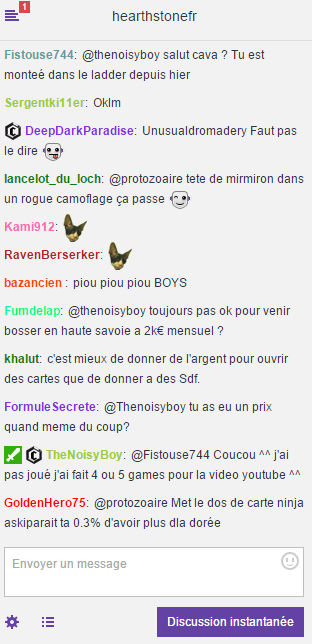
\includegraphics[width=0.8\textwidth]{chatIrc.png}
			\caption{Chat Irc}
		\end{figure}
	\end{columns}	
}
\subsection{Catégorie \& Liste de lectures}
\frame{\frametitle{Catégorie \& Liste de lectures} 
	Les catégories servent à rassembler un certain nombre de vidéos de sites différents.
	
	Les listes de lectures servent à lire à la suite les vidéos quelle contient.
}


\section{Mise en oeuvre}

\subsection{Conception}
\frame{\frametitle{Conception} 
	\begin{figure}[h]
		\center
		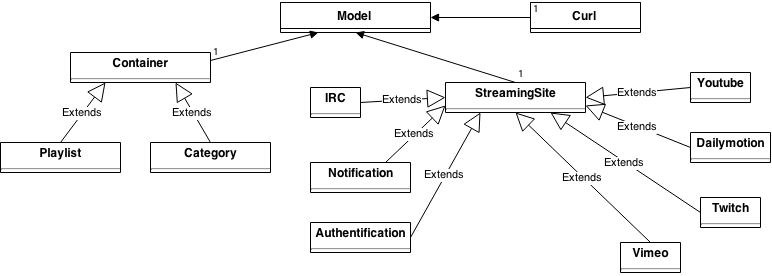
\includegraphics[width=0.6\textwidth]{Model.png}
		\caption{Diagramme}
	\end{figure}
}
\frame{\frametitle{Conception} 
	\begin{figure}[h]
		\center
		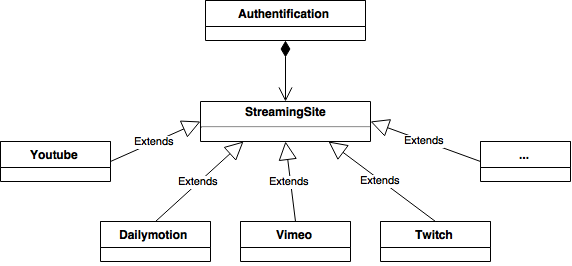
\includegraphics[width=1\textwidth]{StreamingSite.png}
		\caption{Diagramme}
	\end{figure}
}
\subsection{SVideo \& SChannel}
\frame{\frametitle{SVideo \& SChannel}
	\begin{columns}
		\column{0.5\textwidth}
		\begin{itemize}
			\item Structure
				\begin{itemize}
					\item Informations communes
				\end{itemize}
			\item Vidéo et chaîne
			\item Type générique
		\end{itemize}
		
		\column{0.5\textwidth}
		\begin{figure}[h]
			\center
			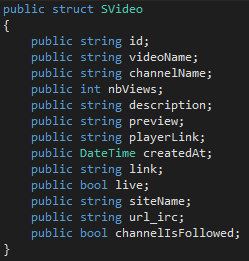
\includegraphics[width=0.8\textwidth]{SVideo.png}
			\caption{Structure vidéo}
		\end{figure}
	\end{columns}
	
	
}

\subsection{Récupération des données}
\frame{\frametitle{Récupération des données} 
	API des différents sites.
	Données reçuent en JSON 
	
	Librarie cURL utilisé : GET, POST, PUT, DELETE
	
	\begin{figure}[h]
		\center
		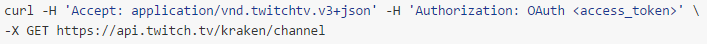
\includegraphics[width=1\textwidth]{curl.png}
		\caption{Commande cURL}
	\end{figure}
}

\frame{\frametitle{Classes structures}
	\begin{columns}
		\column{0.5\textwidth}
		Afin de recevoir les données dans un bon type, il faut créer les classes structures pour chaque sites.
		
		\column{0.5\textwidth}
		\begin{figure}[h]
			\center
			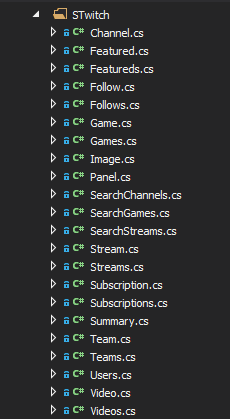
\includegraphics[width=0.5\textwidth]{STwitch.png}
			\caption{Classes Twitch}
		\end{figure}
	\end{columns}
}

\frame{\frametitle{Désérialisation} 
	Type générique et lors de lappel de la methode on indique une classe structure.
	\begin{figure}[h]
		\center
		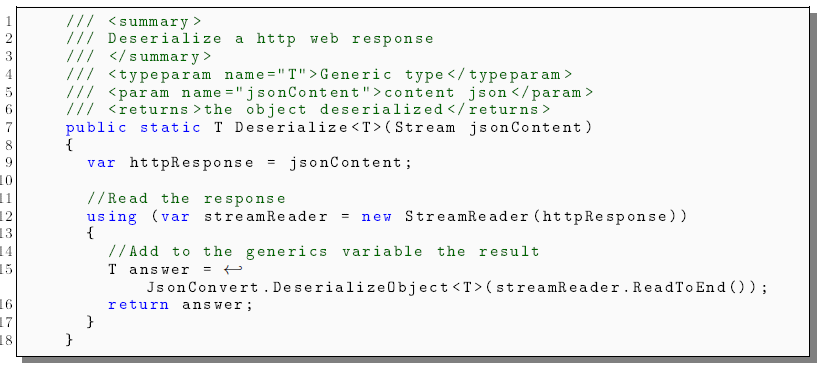
\includegraphics[width=0.9\textwidth]{deserialize.png}
		\caption{Classes Twitch}
	\end{figure}
}

\subsection{Connexion}
\frame{\frametitle{Connexion} 
	\begin{itemize}
		\item Connexion grâce au protocole OAuth2
		\item Utilisation du lien API de connexion
		\begin{itemize}
			\item https ://[url de l'api] ?response\_type=token\&client\_id="[id de l'application]"\& redirect\_uri="[page de redirection]"\&scope="[Liste des droits]"
		\end{itemize}
		\item Récupération du jeton d'accès dans l'url
		\begin{itemize}
			\item Création d'un GitHub Page
		\end{itemize}
	\end{itemize}
	
}

\subsection{Notifications}
\frame{\frametitle{Notifications} 
	Vérification toutes les 5 secondes
	\begin{itemize}
		\item Comparaison de deux listes
		\item Multi-Thread
	\end{itemize}
	
	Composant venant du Web
	\begin{itemize}
		\item NotificationWindow
	\end{itemize}
	
	\begin{figure}[h]
		\center
		
\includegraphics[width=0.7\textwidth]{notificationview.png}
		\caption{Exemple d'une notification}
	\end{figure}
}

\subsection{Catégorie \& liste de lectures}
\frame{\frametitle{Catégorie \& Liste de lectures} 
	Stockage dans un fichier de type INI dans le dossier appdata de l'utilisateur.
	
	Les vidéos sont stockés sous forme de liens.
	\begin{figure}[h]
		\center
		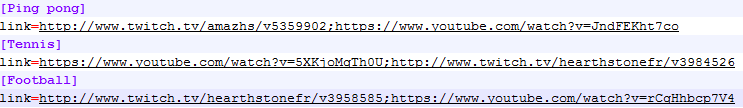
\includegraphics[width=1\textwidth]{inifile.png}
		\caption{Exemple du fichier INI}
	\end{figure}
	
	
}

\section{Conclusion \& perspectives}
\subsection{Conclusions}
\frame{\frametitle{Conclusions} 
	Conclusion technique : 
	\begin{itemize}
		\item Application fonctionnelle
		\item Cahier des charges pas remplit
	\end{itemize}
	
	Conclusion personnelle :
	\begin{itemize}
		\item Plaisant de travailler sur un gros projet
	\end{itemize}	
}

\section{Démonstration} 
\frame{\frametitle{Démonstration} 
}
	
\section{Questions} 
\frame{\frametitle{Questions} 
}
\end{document}

